% BriefCASE tool overview
\todo{Rephrase and clean up - this is mostly copied from IEEE Privacy \& Security paper}

BriefCASE is predicated on a Model-Based Systems Engineering (MBSE) process, in which models are the primary vehicle for communication and understanding among the parties tasked with designing the system. Furthermore, BriefCASE models are the primary design artifacts used for analysis, verification, testing, and code generation.

The BriefCASE tool architecture (see Figure~\ref{fig:briefcase-architecture})) starts with the development of a baseline AADL model of the system. BriefCASE is implemented as a collection of plugins in the Eclipse-based Open Source AADL Tool Environment (OSATE), the reference AADL modeling tool. In OSATE, the AADL system model can be analyzed using any of the supported AADL tools (e.g., resource usage, information flow, latency, and schedulability). 

\begin{figure}[h] 
	\centering 
	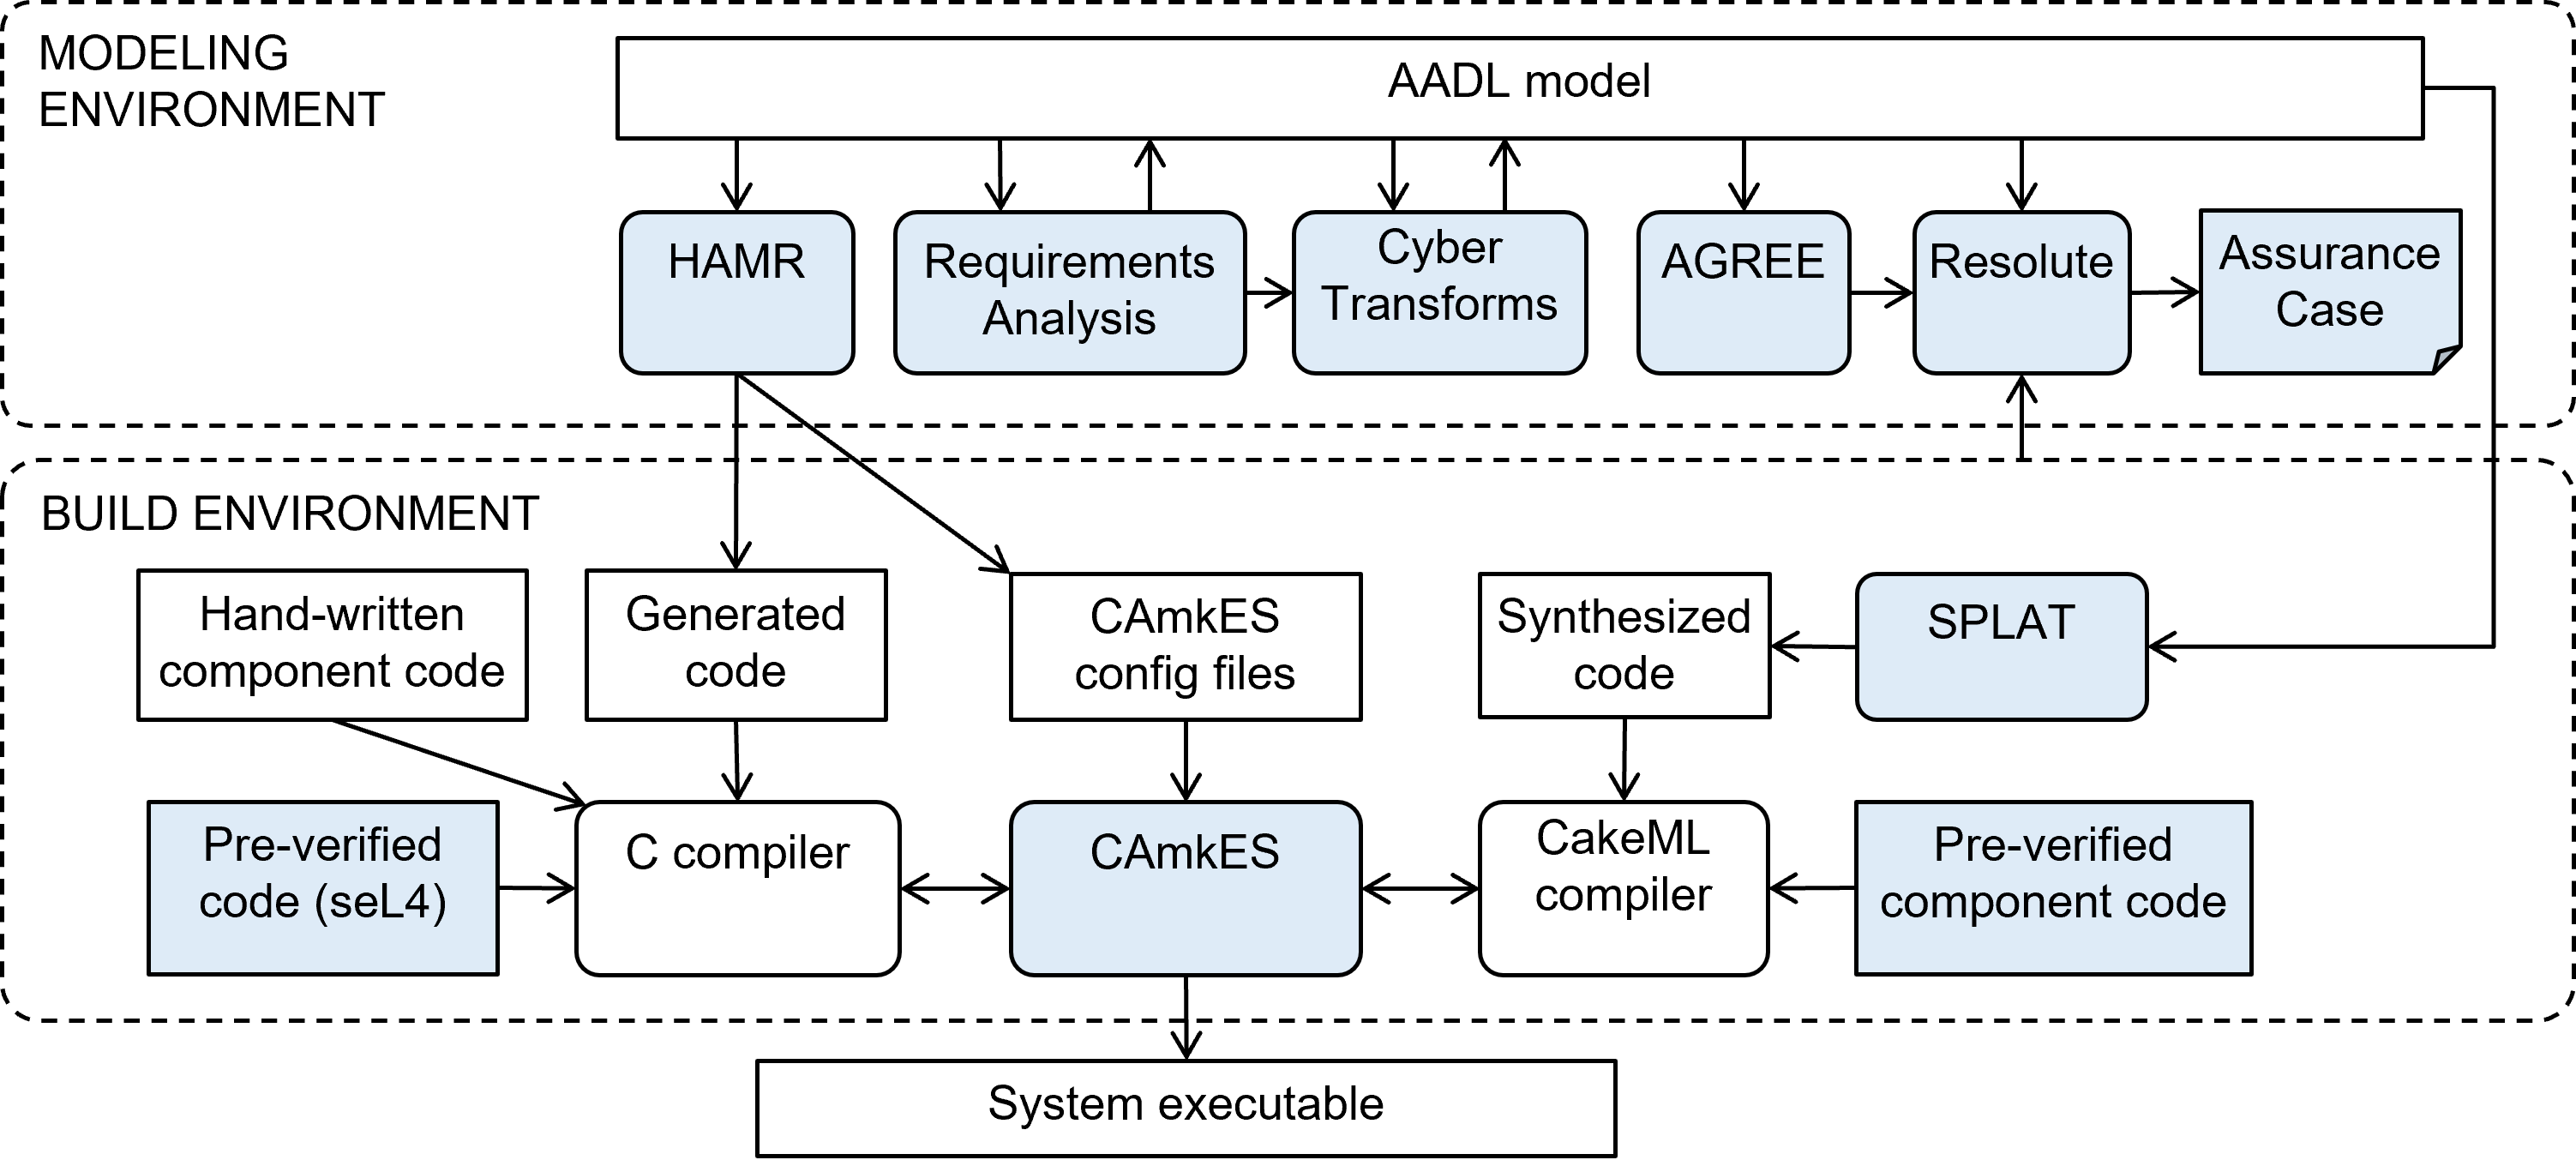
\includegraphics[width=\textwidth]{figs/briefcase-architecture.png}
	\caption{BriefCASE architecture.}
	\label{fig:briefcase-architecture} 
\end{figure}


%	Cyber analysis / Req generation
BriefCASE provides access to two analysis tools (GearCASE [4] and DCRYPPS [5]) that analyze AADL models to detect potential cyber vulnerabilities and suggest requirements for mitigation. 
Systems engineers are presented with a requirements management interface for viewing the generated requirements and importing them into the model so they can be addressed. 
The interface enables engineers to select the requirements they wish to import and assign them unique identifiers, or omit them with rationale. 
A document listing the omitted requirements and rationale is maintained and may be a required development artifact for some certification domains. 
Some requirements can also be formalized as assume-guarantee contracts added to the AADL model, enabling formal verification. Such a requirement will be imported into the model with with an associated formal contract.

A BriefCASE project contains a repository for requirements. Imported requirements are represented as assurance case goals to be satisfied. For example, one of the requirements for well-formed command messages from the ground station (selected in Fig. 3) is imported as the following goal:

The goal is initially marked undeveloped.  Evidential statements are added to the goal as the design is updated to address this requirement.

%	Model transformation
To address the new cyber-resiliency requirement, the architecture will need to be transformed in such a way as to harden the design against the vulnerability. BriefCASE provides an extendable library of model transformations for addressing common cyber vulnerabilities. 

%Currently, the following transformations are supported:
%
%• Filter – Blocks messages that do not conform to the given specification
%• Monitor – Detects violations of a given runtime condition and generates an alert
%• Switch – Used with a Monitor to block messages when an alert is generated (also referred to as a gate)
%• Attestation – Performs a measurement on non-local software to assess its trustworthiness
%• Virtualization – Isolates software component(s) in a virtual machine
%• Proxy – Inserts a pair of components to allow inspection of HTTPS message payloads
%• seL4 – Transforms the model to comply with seL4 component properties 

The transformations are automated by the BriefCASE tool, resulting in a hardened model that is correct-by-construction. 
For example, the requirement that a component only receives well-formed messages can be satisfied by the insertion of a high-assurance filter. A BriefCASE transform wizard helps to configure the filter component properties, including the filter behavioral specification, which is represented as an assume-guarantee contract. BriefCASE then inserts a new filter component into the model, sets the component properties, and establishes the appropriate connections to source and destination components. The filter behavioral contract is also added to the model, enabling formal analysis of the model as well as providing the behavioral specification for a provably correct synthesis of the filter component implementation. 
The transformation also updates the assurance case with new evidential statements indicating that the associated goal has been satisfied, including the strategy used and links to context and
associated evidence.

%	Compositional analysis
The Assume Guarantee Reasoning Environment (AGREE) is a compositional, assume-guarantee-style model checker for AADL models~\cite{compositional-analysis-agree}. AGREE attempts to prove properties about one layer of the architecture using properties allocated to subcomponents. The composition is performed in terms of assumptions and guarantees that are provided for each component. 
%Assumptions describe the expectations the component has on the environment, while guarantees describe bounds on the behavior of the component. 
%AGREE uses k-induction as the underlying algorithm for model checking. AADL models and AGREE contracts are first translated into the Lustre language [7], including verification conditions for consistency and correctness of the contracts. The model checker then attempts to find any model execution traces that would violate these conditions using one of several Satisfiability Modulo Theories (SMT) solvers. If the model checker covers all reachable states in the model without finding a violation then the properties are proved. 
Once the system architecture has been modeled in AADL and the component behavior is specified using AGREE’s assume-guarantee contracts, we use the AGREE model checker to verify the consistency of these contracts.
%
%1) Component interfaces – The output guarantees of each component must be strong enough to satisfy the input assumptions of downstream components.
%
%2) Correctness of implementations – The input assumptions of a system along with the output guarantees of its sub-components must be strong enough to satisfy its output guarantees. 

%For example, in Fig. 1, the input assumptions of the Waypoint Manager must be weaker than the output guarantees of the Geofence monitor and the output guarantees of the Mission Software must be inferrable from its input assumptions combined with the output guarantees of its components. 
This hierarchical strategy for reasoning about contracts, or compositional analysis, reduces the computational complexity of model checking by breaking down the larger problem into more manageable fragments.

%	High-Assurance Component synthesis
The correctness of the high-assurance components inserted by BriefCASE transformations means that each such component must meet its AGREE contract. This obligation is addressed by formal synthesis, using the Semantic Properties of Language and Automata Theory (SPLAT) tool. SPLAT generates code to implement the AGREE contract and then proves that its implementation exactly preserves the meaning of the contract all the way down to the binary for the target platform [8].

SPLAT uses the HOL4 theorem proving system to implement the synthesis and prove its correctness relative to the contract. The synthesis targets a dialect of Standard ML called CakeML and uses CakeML’s fully verified compiler to render the final binary [9]. CakeML is not a real-time language since it is garbage collected, and although that has yet to be an issue in our use cases, it should be considered in applications where strict predictability is required. 

The proof from SPLAT shows equivalence between the contract and the synthesized CakeML and then leverages the existing CakeML compiler proof for the rest. A final step of the proof reasons about the perpetual re-execution of the code as scheduled in a real-time environment. The modeling, relevant properties, and proof of that step is discussed in [10].

%	Infrastructure Code Generation
The High Assurance Modeling and Rapid engineering for embedded systems tool (HAMR) [14] is a multi-platform, multi-language AADL code generation framework. In the CASE project, HAMR is primarily used to generate code for deployment for the seL4 microkernel, but system and component prototyping is also supported utilizing HAMR’s code generation capability for the Java Virtual Machine (JVM) and Linux. 

Using seL4 as a foundation, HAMR enables AADL to be used as a model-based development and systems engineering framework for seL4-based applications. One of the primary objectives is to support system builds that leverage seL4 separation and information flow guarantees to achieve the AADL-specified component isolation and inter-component communication needed for cyber-resiliency. HAMR ensures that seL4 is configured to permit the exact inter-component information flows analyzed and visualized by Awas at the model level.

For each AADL thread component, HAMR generates a thread code skeleton and application programming interfaces (APIs) for communicating over the ports declared on the component. For components that are implemented manually, the developer fills out the thread skeleton with application code. HAMR supports coding component application logic in either C, Slang [15] (a high-assurance subset of Scala that can be translated to C), or CakeML. 

HAMR generates component infrastructure and integration code implementing the semantics of AADL-compliant thread scheduling, thread dispatching, and port-based communication. For port communication, shared memory communication (AADL data ports), buffered messaging (AADL event data ports), and buffered notification (AADL event ports) are supported. HAMR code generation is staged using a translation architecture that facilitates adding new backends for different target platforms. 
%Almost all the infrastructure code is implemented in Slang, which can then be used for JVM deployments or translated to C for Linux or seL4 deployments. The Slang-based implementation of the AADL runtime framework can be viewed as a high-level reference implementation of AADL semantics. Automatic translation of this reference implementation to C on different platforms helps establish semantic consistency across those platforms. 

The seL4 deployment uses the component architecture for microkernel-based embedded systems (CAmkES) code-generation framework to configure the microkernel. The HAMR generated CAmkES directly encodes the AADL model’s component and communication topology and includes the AADL run-time infrastructure with its thread scheduling. HAMR leverages the existing seL4 domain scheduler to enforce time partitioning and provide static cyclic scheduling. 

HAMR also supports Linux-based virtual machine components in the seL4 deployment and the ability to run the entire system on the QEMU emulator. HAMR automatically configures virtual machine based components, and this feature is used to sandbox the untrusted legacy code for the Mission Planner in the example UAV system. The QEMU emulator support facilitates rapid prototyping for test, debug, and analysis, and it enables automated regression testing. 

As part of its code generation process, HAMR produces flow graphs reflecting the inter-component information flow at both the AADL architecture level and the CAmkES level for the seL4 deployment. Visual representations are provided for manual inspection, and SMT-based representations are generated for formal reasoning. The SMT-based representations are used to prove the following properties:

1) All AADL modeled flows are in the CAmkES configuration. 
2) No extraneous flows have been added to the CAmkES configuration. 

These properties focus on cyber-resiliency, but other key semantic properties can be verified as well.

%	Secure Microkernel
The seL4 microkernel [3] is a lightweight, fast, and secure operating system kernel. Its implementation is fully formally verified, from high-level security properties down to the binary level. It was the first OS kernel with this degree of formal verification, and after more than a decade of further research and engineering is still not only the leading formally verified OS kernel, but also the fastest OS kernel on the Arm architecture. 

Its formal verification makes seL4 the ideal basis for high-assurance systems. It is in itself a demonstration of the level of fidelity and scale formal verification can achieve [16]. seL4 supports multiple architectures (Arm, x86-64, RISCV), provides deep security properties such as integrity, confidentiality and availability, and comes with formally verified user-level system initialization. As one of its multiple available OS personalities, seL4 also offers the user-level CAmkES component system that provably achieves isolation between statically specified components. 

The formal proofs about seL4 and the corresponding user-level components measure over one million lines of proof script in total. They constitute one of the largest continually maintained formal proof artifacts in existence and provide a rich target for new techniques in proof engineering, proof repair, and automation for constructing new proofs about software as well as maintaining existing large-scale proof artifacts. 

While it is essential to build a high-assurance system on a high-assurance OS kernel, this is not the main feature seL4 provides for systems engineering — a simpler real-time OS might be formally verified, but would not be sufficient for the engineering method described in this paper. The true power of seL4 lies in its ability to scale formal analysis and verification to the much larger code bases that make up entire systems. It does so by providing strong isolation between user-level components [17].

This isolation means that components can be analyzed separately from each other and be composed safely — in this way seL4 provides the foundation that the soundness of the highly automated analysis tools such as AGREE depend on. It makes it possible to run entire untrusted virtual machines and securely monitor their behavior on the same hardware. It makes it possible to provide filter and monitor components and prove that these components cannot be tampered with by the components they protect. And it makes it possible to guarantee that the limited communication channels that the analysis tools assume to exist in the AADL model are the only communication channels that are available to the components in the system. The combination of these enables automated high-level analysis with high assurance.

% Resolute
%	Very high-level overview of Resolute
%	Maintaining cyber requirements in Resolute
%	Updating requirements with automated transform assurance library in BriefCASE
%	BriefCASE assurance pattern in Resolute
%	Specifying external evidence in Resolute
%	Instantiating and evaluating assurance arguments in Resolute






